\subsubsection{Intervallo di funzionamento strumenti}
Scopo dell'esperienza è la valutazione dell'intervallo di corretta lettura di segnale per i multimetri. \\
Dato il circuito in corrente alternata di figura \ref{fig:C2_P1_circuito}, si misura la tensione ai capi di $Z$ con due strumenti: Multimetro palmare e Oscilloscopio. Si confrontano poi le letture per indivuduare le bande di frequenza in cui la lettura del multimetro risulta corretta.\\
%
Per le correnti viene eseguita la doppia misura con \textcolor{red}{ Multimetro} e Multimetro palmare e, analogamente, vengono confrontati i valori.\\
%
Vengono poi riportati in grafico i rapporti tra le misure effettuate con i due strumenti, $V_{multimetro}/V_{oscilloscopio}$ e $I_{multimetro}/I_{oscilloscopio}$, in funzione della frequenza $\omega$.
%
\paragraph{Nota} {
L'oscilloscopio fornisce letture picco-picco, cioè riporta la differenza di tensione/corrente tra un massimo e un minimo, che è il doppio dell'ampiezza dell'oscillazione di tensione/corrente. Occorre normalizzare per un fattore 1/2 la misura. \\
Il multimetro palmare fornisce letture in RMS, cioè riporta la radice della media quadratica della tensione/corrente sul periodo $T$. Supposta un'oscillazione sinusoidale, $ f(t) = A_0 \sin(\omega t)$, la media quadratica su $[0,T]$ è
    $$\langle f^2(t) \rangle = \frac{1}{T} \; \int_0^{T} A_0^2 \cos^2(\omega t) \mathrm{d}t = \frac{1}{2}A_0^2$$
e la radice:
    $$ \sqrt{ \langle f^2(t) \rangle } = \frac{A_0}{\sqrt{2}}$$
occorre quindi normalizzare il valore per un fattore $\sqrt{2}$.\\
Si è scelto di riportare tutte le quantità in picco-picco.\\
%
\begin{figure}[H]
\centering
\includegraphics[scale=.6]{Grafici/C2_P1_circuito.png}
\caption{Circuito utilizzato.}
\label{fig:C2_P1_circuito}
\end{figure}

\paragraph{Dati e risultati}{
Ddp generata $V_{a}=9.0\pm0.2$ $V$.\\
Resitore per conversione in corrente del segnale in uscita dall'oscilloscopio $R=990\pm20$ $\Omega$. Si riporta in grafico il logaritmo della frequenza $\nu$.
%
    \begin{figure}[H]
        \centering
        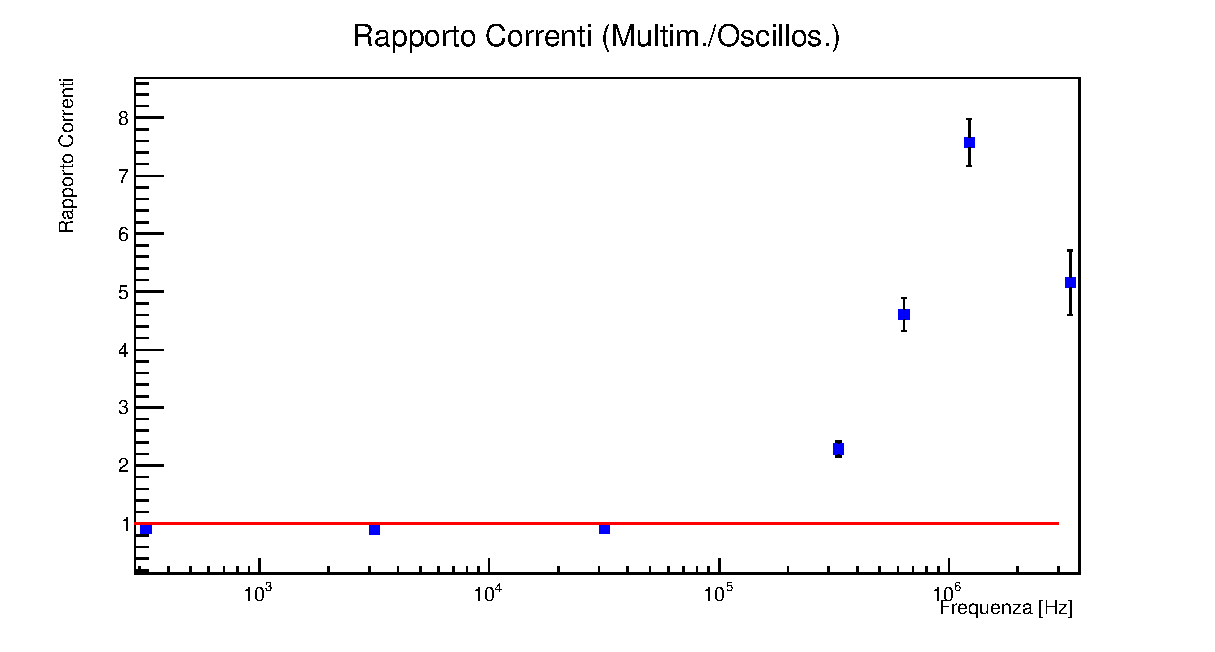
\includegraphics[scale=.6]{Grafici/C2_P1_trueRMS_I.eps}
        \caption{
        Rapporto delle misure di corrente (picco-picco)
        eseguite con multimetro e oscilloscopio per la verifica dell'intervallo di TRUE RMS.
        }
        \label{fig:C2_P1_trueRMS_I}
    \end{figure}
    
    \begin{figure}[H]
        \centering
        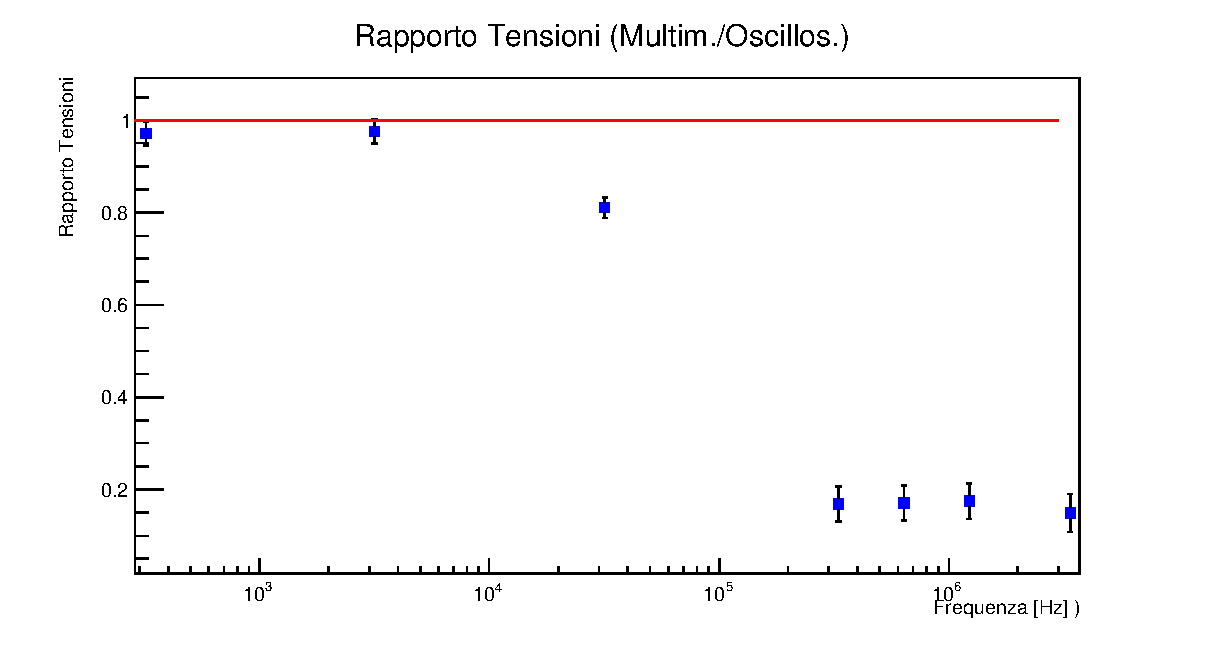
\includegraphics[scale=.6]{Grafici/C2_P1_trueRMS_V.eps}
        \caption{
        Rapporto delle misure di voltaggio (picco-picco) eseguite con multimetro e oscilloscopio per la verifica dell'intervallo di TRUE RMS.
        Usato lo stesso circuito della fig. \ref{fig:C2_P1_trueRMS_I}.
        }
        \label{fig:C2_P1_trueRMS_V}
    \end{figure}
    
}%}

\paragraph{Conclusioni}{
Si può notare che l'intervallo di funzionamento ottimale del multimetro palmare comprende le frequenze fino all'ordine dei $10 kHz$.
}

\subsubsection{Impedenza}
Scopo dell'esperienza è valutare modulo e fase dell'impedenza per un resistore in un circuito solo resistivo.\\
Per un componente resistivo, l'impedenza ha solamente parte reale con $Z=R_Z$, quindi si ha $Mod(Z) = R_Z$ e $Arg(Z) = 0 $. Per determinare il valore della resistenza, si applica la legge di Ohm, dove si indica con $Z$ l'impedenza (resistenza) relativa al resistore da misurare e con $R$ la resistenza di prova per la misura della corrente ($R=1kOhm$). 
    $$ Z = V/I = \frac{V_{b-a} }{V_b/R} $$
    %
Noto il valore di $Z=15.97 k\Omega$ (misurato con multimetro), i dati riportano (si osservi l'ultima riga della tabella \ref{tab:C2_P1_trueRMS} per i valori della fase $\Delta \phi(V_ab - I_b)$.
%
    \begin{figure}[H]
        \centering
        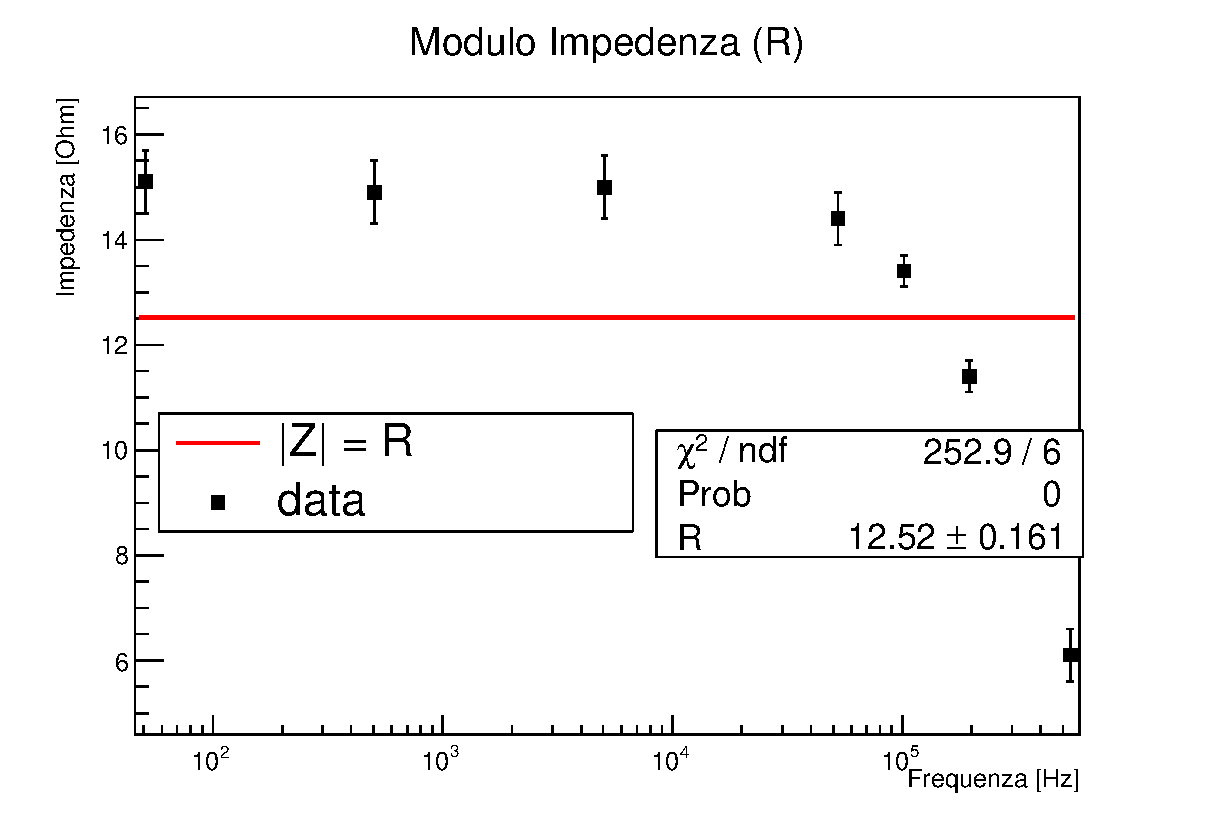
\includegraphics[scale=.7]{Grafici/C2_P1_impedenzaR.eps}
        \caption{Dati relativi al modulo dell'impedenza}
    \end{figure}
%
\paragraph{Considerazioni}{Per quanto riguarda il modulo dell'impedenza, dal fit risulta $ 12.5 \pm 0.2 k\Omega$, ben lontano dal valore misurato con il multimetro, mentre per la fase si osserva che assume valori non nulli ad alte frequenze. Si attribuisce l'effetto a eventuali componenti non resistive degli strumenti di misura, o a malfuzionamento.}
\subsubsection{Tabelle dati}
    \begin{table}[H]
\begin{center}
\begin{tabular}{|c|c|c|c|c|c|c|c|c|}
\hline
\multicolumn{9}{|c|}{ \textbf{Generatore di funzioni} } \\ \hline
%
Freq & Hz $\pm 2$\% & 50.8 & 504 & 5.10 k & 52.6 k & 101 k & 195 k & 537 k \\ \hline
%
\multicolumn{9}{c}{}\\
\hline
\multicolumn{9}{|c|}{ \textbf{Multimetro palmare - Fluke 115} }\\ \hline
V rms & V & 2.86 & 2.87 & 2.45 & 0.5 & 0.5 & 0.5 & 0.4 \\ 
 & $\pm$ err & 0.01 & 0.01 & 0.01 & 0.1 & 0.1 & 0.1 & 0.1 \\ \hline
V pp & V & 8.09 & 8.12 & 6.93 & 1.4 & 1.4 & 1.4 & 1.1 \\ 
 & $\pm$ err & 0.03 & 0.03 & 0.03 & 0.3 & 0.3 & 0.3 & 0.3 \\
%
\hline
\multicolumn{9}{c}{}\\
\hline
\multicolumn{9}{|c|}{ \textbf{Multimetro - HP 34401A} }\\ \hline
I rms & $\mu$ A & 181.0 & 181.0 & 188.0 & 474 & 1020 & 1920 & 2210 \\ 
 & $\pm$ err & 0.1 & 0.1 & 0.1 & 1 & 10 & 10 & 10 \\ \hline
I pp & $\mu$ A & 512 & 511.8 & 530.6 & 1341 & 2890 & 5430 & 6250 \\
 & $\pm$ err & 0 & 0.3 & 0.3 & 3 & 30 & 30 & 30 \\\hline
\multicolumn{9}{c}{}\\
\hline
\multicolumn{9}{|c|}{ \textbf{Oscilloscopio - Tektronik tds 220} }\\ \hline
Va & V & 8.9 & 8.9 & 9.1 & 9.0 & 8.9 & 8.8 & 8.8 \\ 
 & $\pm$ err & 0.2 & 0.2 & 0.2 & 0.2 & 0.2 & 0.2 & 0.2 \\ \hline
Vb & V & 0.55 & 0.56 & 0.57 & 0.58 & 0.62 & 0.71 & 1.2 \\ 
 & $\pm$ err & 0.02 & 0.02 & 0.02 & 0.02 & 0.02 & 0.02 & 0.1 \\ \hline
$V(b-a)$ & V & 8.3 & 8.3 & 8.6 & 8.4 & 8.3 & 8.1 & 7.6 \\ 
 & $\pm$ err & 0.2 & 0.2 & 0.2 & 0.2 & 0.2 & 0.2 & 0.2 \\ \hline
$ Ib = Vb/R $ & $\mu$ A & 0.56 & 0.57 & 0.58 & 0.59 & 0.63 & 0.72 & 1.21 \\
 & $\pm$ err\% & 6\% & 6\% & 6\% & 5\% & 5\% & 5\% & 10\% \\ 
%
\hline
\multicolumn{9}{c}{}\\
\hline
%
\multicolumn{9}{|c|}{\textbf{Differenze di fase}}\\\hline
$\Delta\phi' (Va-Vb) $  & ns        & 0 & 0 & 0 & 800 & 600 & 440 & 250 \\
                        & $\pm$err  & 0 & 0 & 0 & 100 & 100 & 40  & 10  \\
\hline
$\Delta\phi (Vab - Ib)$ & ns        & 0 & 0 & 0 & 1400 & 1400 & 1200 & 710 \\ 
                        & $\pm$err  & 0 & 0 & 0 & 200  & 100  & 40   & 10  \\
\hline

\end{tabular}
\end{center}
\caption{
Dati relativi ai grafici delle figure \ref{fig:C2_P1_trueRMS_I} e \ref{fig:C2_P1_trueRMS_V}.
Resitore $R=990\pm20$ $\Omega$.
$T=1/\nu$ indica il periodo.
}
\label{tab:C2_P1_trueRMS}
\end{table}
